\section{SampleClean \cite{wang1999sample}}
This section introduces the basic SampleClean framework where the results of aggregate queries on dirty relations are estimated and bounded. The subsequent variants of the problem will build on the formalization and results of this section.

\subsection{Problem Setup}

\noindent \textbf{Dirty Relation: } Let $R$ be a dirty relation, where it is corrupted with the following errors: (\emph{Attribute Errors}) a row $r\in R$ has an attribute error in an attribute $a$ if $r(a)$ is incorrect or has a missing value,  (\emph{Duplication Errors} ) a row $r \in R$ is said to be a duplicate if there exists another distinct $r' \in R$ such that they refer to the same entity.

\vspace{.25em}

\noindent For every dirty relation $R$, there is a cleaned version $R_{clean}$ where attribute errors are corrected (or filled) and duplicates are merged to a canonical version. 

\vspace{.25em}

\noindent\textbf{Data Cleaning Model: } 
For each row $r \in R$ the user-specified data cleaning technique must provide returns the following quantities: (\Correct{r}[a]) the corrected value of the attribute, (\Dedup{r}{R}) the number of times the record is duplicated in the entire dataset.

\vspace{.25em}

\noindent\textbf{Queries: } SampleClean addresses aggregate queries of the form:
\begin{alltt}
SELECT \textsf{f}(a) FROM R WHERE predicate GROUP BY gb_attrs
\end{alltt}
where f is \avgfunc, \sumfunc, or \countfunc. 

\vspace{.25em}

\begin{problem}[Sample-and-Clean]
Given a dirty relation $R$, and a user-specified data cleaning function $C(\cdot)$, the Sample-and-Clean problem is to estimate the result of an aggregate query $q$ applied to the hypothetical cleaned relation $q(R_{clean})$ with a budget of applying $C$ to at most $k$ rows of $R$. 
\end{problem}

\subsection{Sample Estimates}\label{subsec:resultestimation}
Consider a simpler problem; suppose we want to estimate the \mean value of $R$ ignoring data error from a sample $S$.
If $S$ is a sample uniformly at random from $R$ (with or without replacement), we can calculate the \mean of $S$ and for a large enough sample, the Central Limit Theorem (CLT) states that these estimates follow a normal distribution:
\[\small
N(\mean(R),\frac{var(R)}{k})
\]
Since the estimate is normally distributed, we can define a confidence interval parametrized by $\lambda$ (e.g., 95\% indicates $\lambda=1.96$)\footnote{\scriptsize When estimating means from samples without replacement there is a finite population correction factor of $FPC=\frac{N-k}{N-1}$ which scales the confidence interval.}.
\begin{equation}\small
\mean(S) \pm \lambda \sqrt{\frac{var(S)}{k}}.
\end{equation}

We can reformulate all of the queries as calculating a \mean value so we can estimate their confidence intervals with the CLT 
$
f(S) = \frac{1}{k} \sum_{r \in S} \saqpfunc(r)
$.
where $\saqpfunc(\cdot)$\footnote{\Predicate{t} is the predicate of the aggregate query, where \Predicate{t} = 1 or 0 denotes $r$ satisfies or dissatisfies the predicate, respectively. $k_{\pred}$ is the number of tuples that satisfy the predicate in the sample.} expresses all of the necessary scaling to translate the query into a \mean value calculation:
\begin{itemize}\vspace{-.5em}
\item \countfunc: $\saqpfunc(t) = \Predicate{r} \cdot N$\vspace{-.5em}
\item \sumfunc: ~\, $\saqpfunc(t) = \Predicate{r} \cdot N \cdot r(a)$\vspace{-.5em}
\item \avgfunc: ~\, $\saqpfunc(t) = \Predicate{r} \cdot \frac{k}{k_{\pred}}  \cdot r(a) $ 
\end{itemize}

\subsection{Direct Estimation with Data Errors}
We are interested in estimating an aggregate query on $R_{\clean}$.
However, since we do not have the clean data, we cannot directly sample from $R_{\clean}$.
We must draw our sample from the dirty data $R$ and then clean the sample.

Running an aggregate query on the cleaned sample is not equivalent to computing the query result on a sample directly drawn from the clean data.
Consider the case where data is duplicated, sampling from the dirty data leads to an overrepresentation of the duplicated data in the sample.
Even if cleaning is subsequently applied it does not change the fact that the sample is not uniform; and thus, the estimation method without errors presented before does not apply.
Our goal is to define a new function $\saqpplusfunc(\cdot)$, an analog to $\saqpfunc(\cdot)$, that corrects attribute values and re-scales to ensures that the estimate remains unbiased.

\subsubsection{Attribute Errors}
This sampling statistics change only affected duplication errors, attributes errors only affects an individual row.
Consequently, if we apply the $\saqpfunc(\cdot)$ to the corrected tuple, we still preserve the uniform sampling properties of the sample $S$.
In other words, the probability that a given tuple is sampled is not changed by our correction of value and condition errors, thus we define $\saqpplusfunc(t)$ as:
\[\small
\saqpplusfunc(t) = \saqpfunc \left( \Correct{t} \right).
\]
Note that the $\saqpfunc(\cdot)$ for an \avgfunc query is dependent on the parameter $k_{\pred}$. 
If we correct values in the predicate attributes, we need to recompute $k_{\pred}$ in the cleaned sample.

\subsubsection{Duplication Errors}
Since duplication errors affect multiple tuples and the size of $R_{\clean}$ is different from the size of $R$, they do affect the uniformity of the sampling.
The duplicated data is more likely to be sampled and thus be over-represented in the estimate of the \mean.
We can address this with a weighted mean to reduce the effects of this over-representation.
Furthermore, we can incorporate this weighting into $\saqpplusfunc(\cdot)$.

Specifically, if a tuple $r$ is duplicated $m=\Dedup{r}{R}$ times, then it is $m$ times more likely to be sampled, and we should down weight it with a $\frac{1}{m}$ factor compared to the other tuples in the sample.
We formalize this intuition with the following lemma (proved in \cite{wang1999sample}):
\begin{lemma}\label{lem:derror}
Let $R$ be a population with duplicated tuples. % and $P_{unique}$ be the set of unique tuples.
Let $S \subseteq R$ be a uniform sample of size $k$.
For each $r_{i}\in S$, let $m_i$ denote its number of duplicates in $R$.
 (1) For \sumfunc and \countfunc queries, applying $\saqpplusfunc(r_i)=\frac{\saqpfunc(r_i)}{m_i}$ yields an unbiased estimate;
(2) For an \avgfunc query, the result has to be scaled by the duplication rate $d=\frac{k}{k'}$,
where $k'=\sum_i\frac{1}{m_i}$, so using $\saqpplusfunc(r_i)=d\cdot\frac{\saqpfunc(r_i)}{m_i}$ yields an unbiased estimate.
\end{lemma}

\subsubsection{Summary and Algorithm}
In Table \ref{tbl:transform-new}, we describe the transformation $\saqpplusfunc(\cdot)$.
Using this function, we formulate the direct estimation procedure:

\begin{enumerate}
\item Given a sample $S$ and an aggregation function $f(\cdot)$\vspace{-.5em}
\item Apply $\saqpplusfunc(\cdot)$ to each $t_i \in S$ and call the resulting set $\saqpplusfunc(S)$\vspace{-.5em}
\item Calculate the mean $\mu_c$, and the variance $\sigma_c^2$ of $\saqpplusfunc(S)$\vspace{-.5em}
\item Return $\mu_c \pm \lambda \sqrt{\frac{\sigma_c^2}{K}}$\vspace{-.5em}
\end{enumerate}

\begin{table}[tup]\vspace{-1em}

\small
\caption{$\saqpplusfunc(\cdot)$ for \countfunc, \sumfunc, and \avgfunc. Note that $N$ is the total size of dirty data (including duplicates).}
\centering 
\begin{tabular}{l l}
\hline\hline
Query & $\saqpplusfunc(\cdot)$\\
\hline  % inserts single horizontal line
\vspace{.5em}
$\countfunc$ & $
		\Predicatec{r}\cdot N\cdot\frac{1}{\Dedup{r}{R}}
$ \\\vspace{.5em} % inserting body of the table
$\sumfunc$ & $
		\Predicatec{r}\cdot N\cdot\frac{\Correct{r}[a]}{\Dedup{r}{R}}
$ \\\vspace{.5em}
$\avgfunc$ & $
		\Predicatec{t}\cdot \frac{dk}{k_{\pred}}\cdot\frac{\Correct{r}[a]}{\Dedup{r}{R}}
$ \\ [1ex] % [1ex] adds vertical space
\hline %inserts single line 
\label{tbl:transform-new}
\end{tabular}\vspace{-2em}
\end{table}

\subsection{Correction with Data Errors}
Due to data errors, the result of the aggregation function~$f$ on the dirty population $R$ differs from the true result $f(R) = f(R_{\clean}) + \epsilon$.
We derived a function $\saqpplusfunc(\cdot)$ for the direct estimation.
We contrasted this function with $\saqpfunc ( \cdot )$ which does not clean the data.
Therefore, we can write:
\[
f(R) = \frac{1}{N}\sum_{r\in R}\saqpfunc(r)\hspace{2em}
f(R_{\clean}) = \frac{1}{N}\sum_{r\in R}\saqpplusfunc(t)
\]
If we solve for $\epsilon$, we find that:
\[
\epsilon = \frac{1}{N}\sum_{r\in R}\Big(\saqpfunc(r)-\saqpplusfunc(r)\Big)
\]
In other words, for every tuple r, we calculate how much $\saqpplusfunc(r)$ changes $\saqpfunc(r)$.
For a sample $S$, we can construct the set of differences between the two functions:
\[\scriptsize
Q=\{\saqpfunc(r_1)-\saqpplusfunc(r_1),\saqpfunc(r_2)-\saqpplusfunc(r_2), \cdots ,\ \saqpfunc(r_K)-\saqpplusfunc(r_K)\}\]
The \mean difference is an unbiased estimate of $\epsilon$, the difference between $f(R)$ and $f(R_{\clean})$.
We can subtract this estimate from an existing aggregation of data to get an estimate of $f(R_{\clean})$.

We derive the correction estimation procedure, which corrects an aggregation result:
\begin{enumerate}
\item Given a sample $S$ and an aggregation function $f(\cdot)$
\item Apply $\saqpfunc(\cdot)$ and $\saqpplusfunc(\cdot)$ to each $r_i \in S$ and call the set of differences  $Q(S)$.
%Set $s_i$ to zero if the tuple does not satisfy the predicate in the dirty data.
\item Calculate the mean $\mu_q$, and the variance $\sigma_q$ of $Q(S)$
\item Return $(f(R) - \mu_q) \pm \lambda \sqrt{\frac{\sigma_q^2}{k}}$
\end{enumerate}

\subsection{Analysis}
\noindent \textbf{Direct Estimate vs. Correction: } In terms of the confidence intervals, we can analyze how direct estimation compares to correction for a fixed sample size $k$.
\sloppy
direct estimation gives an estimate that is proportional to the variance of the clean sample view:  $\frac{\sigma_{c}^2}{k}$.
Correction gives and estimate proportional to the variance of the \emph{differences} before and after cleaning: $\frac{\sigma_{q}^2}{k}$.
$\sigma_{q}^2$ can be rewritten as
\[\sigma_{c}^2 + \sigma_{q}^2 - 2cov(S,S_{clean})\]
$cov(S,S_{clean})$ is the covariance between the the variables $\saqpfunc(r)$ and $\saqpplusfunc(r)$.
Therefore, a correction will have less variance when:
\[\sigma_{S}^2 \le 2cov(S,S_{clean})\]
If there are no errors $S_{clean} = S$ and then $cov(S,S_{clean})=\sigma_c^2$ clearly satisfying the condition.
Generally, if errors are small (i.e., the cleaned data is highly correlated with the dirty data) corrections will give higher accuracy.
In practice, we can run both the correction and the direct estimate and take the one with a narrower confidence interval:
\begin{equation}
error^2 \le O(\frac{\min\{\sigma_c^2,\sigma_q^2\}}{k})
\end{equation}

\vspace{0.5em}

\noindent \textbf{Selectivity: }
Let $p$ be the selectivity of the query and $k$ be the sample size; that is, a fraction $p$ records from the relation satisfy the predicate.
For these queries, we can model selectivity as a reduction of effective sample size $k\cdot p$ making the
estimate variance: $O(\frac{1}{k*p})$.
Thus, the confidence interval's size is scaled up by $\frac{1}{\sqrt{p}}$.
Just like there is a tradeoff between accuracy and maintenance cost, for a fixed accuracy, 
there is also a tradeoff between answering more selective queries and maintenance cost.

\subsection{Results: Ranking Academic Authors}
Microsoft maintains a public database of academic publications\footnote{\scriptsize http://academic.research.microsoft.com (Accessed Nov. 3, 2013)}.
The errors in this dataset are primarily duplicated publications and mis-attributed publications.
We selected publications from three database researchers: Jeffrey Ullman, Michael Franklin, and Rakesh Agarwal.
To clean a sample of publications, we first manually removed the mis-attributions in the sample. Then, we applied the technique used in~\cite{DBLP:journals/pvldb/WangKFF12} to identify potential duplicates for all of publications in our sample, and manually examined the potential matches.  
For illustration purpose, we cleaned the entire dataset, and showed the cleaning results in Table~\ref{tbl:dataset:ms-academic}. 
\begin{table}[!ht]\vspace{-1em}
\centering\caption{Microsoft Academic Search Dataset.}\vspace{.5em} \label{tbl:dataset:ms-academic}
\begin{tabular}{r r r r r}
\hline\hline
Name & Dirty & Clean & Pred \% & Dup \\ 
\hline  % inserts single horizontal line
Rakesh Agarwal & 353 & 211 & 18.13\% & 1.28\\
\hline
Jeffery Ullman & 460 & 255 & 05.00\% & 1.65\\
\hline
Michael Franklin & 560 & 173 & 65.09\% & 1.13\\
\hline
%\hline %inserts single line
\end{tabular}\vspace{-.75em}
%\reminder{May be we need to save some space.}
%\caption{The Microsoft Academic Search Dataset. We manually cleaned the datasets for each of the authors.
%This table shows the difference between the reported number of publications (AllDirty) and the number of publications after our cleaning (AllClean).
%We also include the false positive percentage and the duplication ratio (Section \ref{sec:sampleclean}) to illustrate the type of errors.}\label{dataset:ms-academic}\vspace{-1em}
\end{table}

This table shows the difference between the reported number of publications (Dirty) and the number of publications after our cleaning (Clean).
We also diagnosed the errors and recorded the duplication ratio (Dup) and the percentage of mis-attributed papers (Pred).
Both Rakesh Agarwal and Michael Franklin had a large number of mis-attributed papers due to other authors with the same name (64 and 402 respectively).
Jeffery Ullman had a comparatively larger number of duplicated papers (182).

If we were interested in ranking the authors, the dirty data would give us the wrong result. 
In Figure \ref{exp:ms-academic-ranking}, we plot the probablity of incorrect ranking as a function of number of cleaned records with SampleClean.
We show how we can return the correct ranking with 95\% probability after cleaning only 210 total samples.
To achieve a correct ranking with 99\% probability, we require 326 samples to be cleaned.
In comparison, AllDirty always returns an incorrect ranking.
SampleClean provides a flexible way to achieve a desired confidence on decision based on dirty data queries.

\begin{SCfigure}
%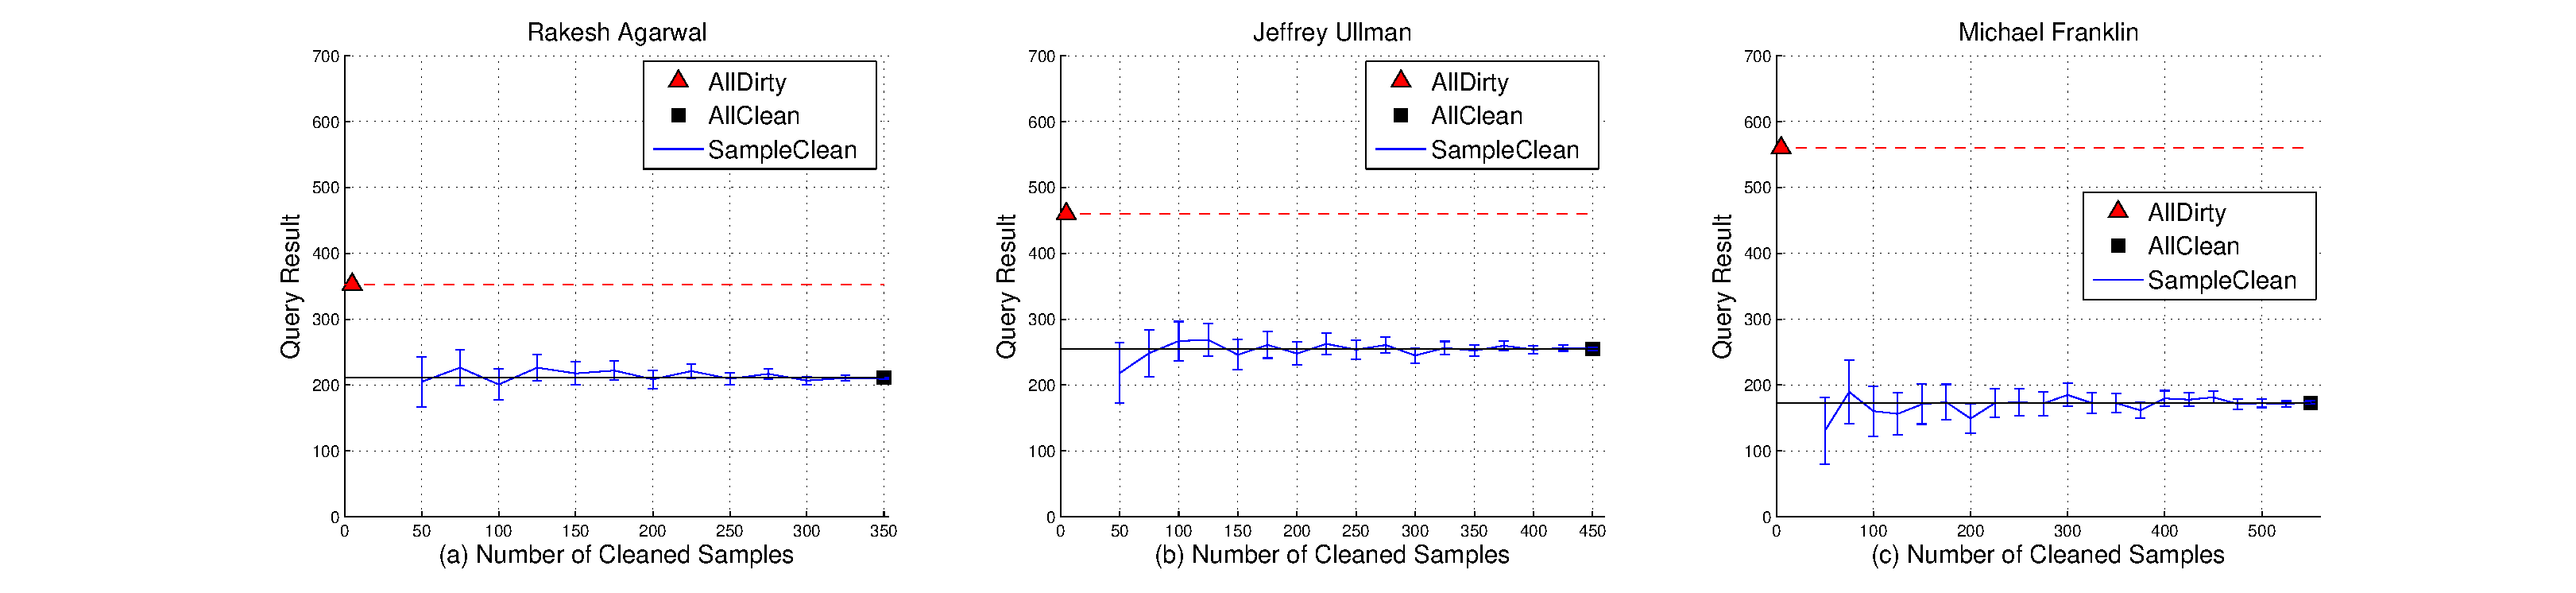
\includegraphics[width=0.78\textwidth]{figs/msacademic-paper-count.eps}
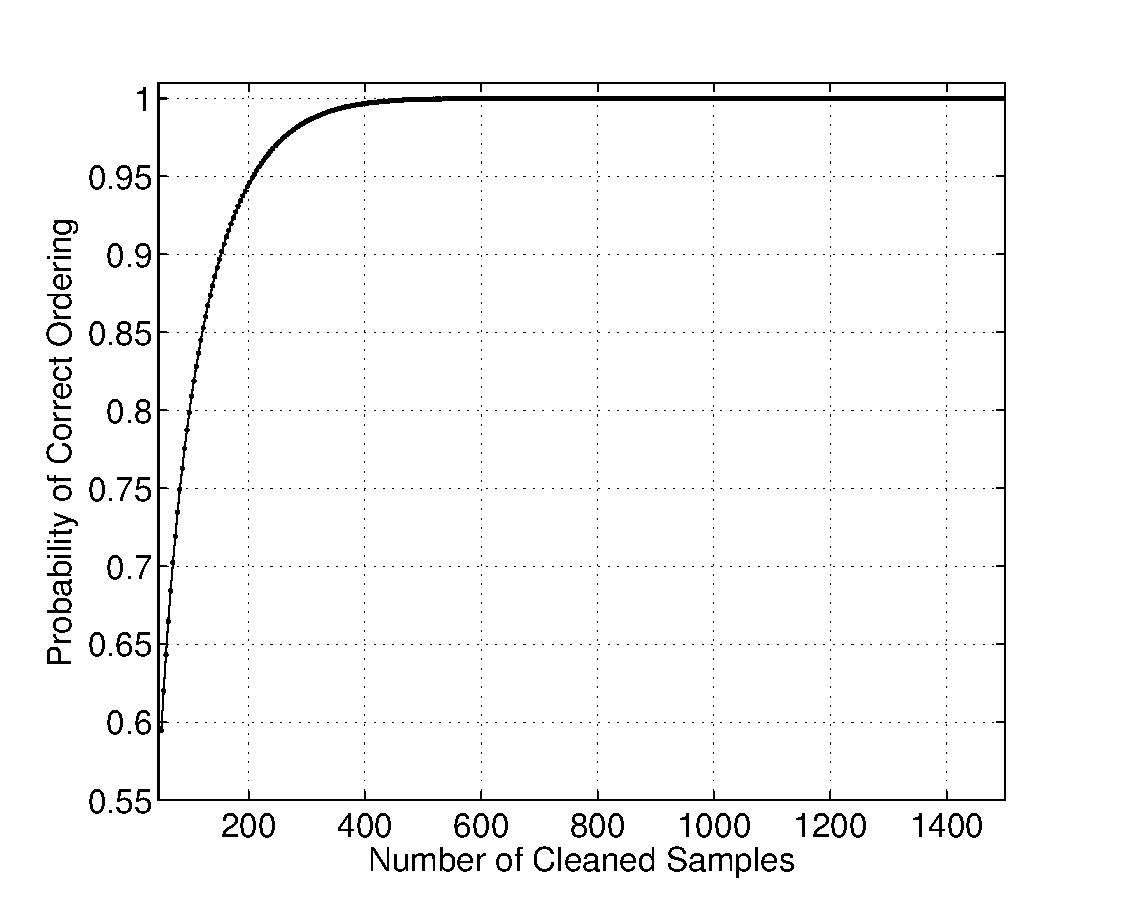
\includegraphics[width=0.3\textwidth]{figs/msacademic-paper-ranking.eps}
\caption{Even though the dirty result always returns an incorrect ranking, we can return the correct ranking with 95\% probability after cleaning only 210 total samples. To achieve a correct ranking with 99\% probability, we require 326 samples to be cleaned.\label{exp:ms-academic-ranking}}

\end{SCfigure}


